% Options for packages loaded elsewhere
\PassOptionsToPackage{unicode}{hyperref}
\PassOptionsToPackage{hyphens}{url}
%
\documentclass[
  10pt,
]{article}
\usepackage{lmodern}
\usepackage{amssymb,amsmath}
\usepackage{ifxetex,ifluatex}
\ifnum 0\ifxetex 1\fi\ifluatex 1\fi=0 % if pdftex
  \usepackage[T1]{fontenc}
  \usepackage[utf8]{inputenc}
  \usepackage{textcomp} % provide euro and other symbols
\else % if luatex or xetex
  \usepackage{unicode-math}
  \defaultfontfeatures{Scale=MatchLowercase}
  \defaultfontfeatures[\rmfamily]{Ligatures=TeX,Scale=1}
\fi
% Use upquote if available, for straight quotes in verbatim environments
\IfFileExists{upquote.sty}{\usepackage{upquote}}{}
\IfFileExists{microtype.sty}{% use microtype if available
  \usepackage[]{microtype}
  \UseMicrotypeSet[protrusion]{basicmath} % disable protrusion for tt fonts
}{}
\makeatletter
\@ifundefined{KOMAClassName}{% if non-KOMA class
  \IfFileExists{parskip.sty}{%
    \usepackage{parskip}
  }{% else
    \setlength{\parindent}{0pt}
    \setlength{\parskip}{6pt plus 2pt minus 1pt}}
}{% if KOMA class
  \KOMAoptions{parskip=half}}
\makeatother
\usepackage{xcolor}
\IfFileExists{xurl.sty}{\usepackage{xurl}}{} % add URL line breaks if available
\IfFileExists{bookmark.sty}{\usepackage{bookmark}}{\usepackage{hyperref}}
\hypersetup{
  pdftitle={World Cup Qatar 2022 groupstage predictions: 3rd match day},
  pdfauthor={Leonardo Egidi, Vasilis Palaskas - Mail: legidi@units.it, vasilis.palaskas94@gmail.com},
  hidelinks,
  pdfcreator={LaTeX via pandoc}}
\urlstyle{same} % disable monospaced font for URLs
\usepackage[margin=1in]{geometry}
\usepackage{longtable,booktabs}
% Correct order of tables after \paragraph or \subparagraph
\usepackage{etoolbox}
\makeatletter
\patchcmd\longtable{\par}{\if@noskipsec\mbox{}\fi\par}{}{}
\makeatother
% Allow footnotes in longtable head/foot
\IfFileExists{footnotehyper.sty}{\usepackage{footnotehyper}}{\usepackage{footnote}}
\makesavenoteenv{longtable}
\usepackage{graphicx,grffile}
\makeatletter
\def\maxwidth{\ifdim\Gin@nat@width>\linewidth\linewidth\else\Gin@nat@width\fi}
\def\maxheight{\ifdim\Gin@nat@height>\textheight\textheight\else\Gin@nat@height\fi}
\makeatother
% Scale images if necessary, so that they will not overflow the page
% margins by default, and it is still possible to overwrite the defaults
% using explicit options in \includegraphics[width, height, ...]{}
\setkeys{Gin}{width=\maxwidth,height=\maxheight,keepaspectratio}
% Set default figure placement to htbp
\makeatletter
\def\fps@figure{htbp}
\makeatother
\setlength{\emergencystretch}{3em} % prevent overfull lines
\providecommand{\tightlist}{%
  \setlength{\itemsep}{0pt}\setlength{\parskip}{0pt}}
\setcounter{secnumdepth}{-\maxdimen} % remove section numbering
\usepackage{color}
\usepackage{bm}

\title{World Cup Qatar 2022 groupstage predictions: 3rd match day}
\author{Leonardo Egidi, Vasilis Palaskas - Mail:
\href{mailto:legidi@units.it}{\nolinkurl{legidi@units.it}},
\href{mailto:vasilis.palaskas94@gmail.com}{\nolinkurl{vasilis.palaskas94@gmail.com}}}
\date{28 November 2022}

\begin{document}
\maketitle

{
\setcounter{tocdepth}{2}
\tableofcontents
}
\hypertarget{the-statistical-model-in-brief}{%
\section{The statistical model (in
brief)}\label{the-statistical-model-in-brief}}

We use a \textbf{diagonal-inflated Bivariate-Poisson model with dynamic
team-specific abilities} for the attack and the defence. Let
\((X_{i}, Y_{i})\) denote the random number of goals scored by the home
and the away team in the \(i\)-th game, \(i=1,\ldots,n\), respectively.
\(\mathsf{ranking}\) denotes the Coca-Cola FIFA ranking at October 6th,
2022, whereas att and def denote the attack and the defence abilities,
respectively.

\begin{align}
(X_i, Y_i) &\ \sim \ \begin{cases} (1-p) \text{BP}(x_i, y_i |\lambda_1, \lambda_2, \lambda_3) \ \ \ & \text{if} \    x \ne y \\ (1-p) \text{BP}(x_i, y_i | \lambda_1, \lambda_2, \lambda_3) + pD(x, \eta) \ \ \ & \text{if} \   x = y, \end{cases}, \\
\log(\lambda_{1i}) &=\    \text{att}_{h_i, t}+ \text{def}_{a_i,t} + \frac{\gamma}{2}(\mathsf{ranking}_{h_i}-\mathsf{ranking}_{a_i}) \\
\log(\lambda_{2i}) & =\    \text{att}_{a_i,t} + \text{def}_{h_i,t} - \frac{\gamma}{2}(\mathsf{ranking}_{h_i}-\mathsf{ranking}_{a_i}), \ \ i=1,\ldots,n\ (\text{matches}), \\
\log(\lambda_{3i}) & =\ \rho,\\
\text{att}_{k, t}&  \sim \ \mathcal{N}(\text{att}_{k, t-1}, \sigma^2), \\
\text{def}_{k, t} & \sim \  \mathcal{N}(\text{def}_{k, t-1}, \sigma^2),\\
\rho, \ \gamma & \sim \mathcal{N}(0,1) \\
p & \sim \text{Uniform}(0,1)\\
& \sum_{k=1}^{n_t} \text{att}_{k, }=0, \  \sum_{k=1}^{n_t}\text{def}_{k, }=0, \ \ k=1,\ldots n_t \ (\text{teams}), \  t=1,\ldots, T \ (\text{times}).
\label{eq:scoring_rue}
\end{align}

Lines (1) displays the likelihood's equations (diagonal inflated
bivariate Poisson); lines (2)-(4) display the log-linear models for the
scoring rates \(\lambda_{1}, \lambda_{2}\) and the covariance parameter
\(\lambda_3\); lines (5)-(6) display the dynamic prior distributions for
the attack and the defence parameters, respectively; lines (7)-(8)
display prior distributions for the other model parameters; line (9)
displays the sum-to-zero identifiability constraints. Model fitting has
been obtained through the Hamiltonian Monte Carlo sampling, 2000
iterations, 4 chains using the \texttt{footBayes} \texttt{R} package
(with the underlying \texttt{rstan} package). The historical data used
to fit the models come from \emph{all the international matches played
during the years' range 2018-2022}.

The idea is to provide a dynamic predictive scenario: at the end of each
match-day, the model will be refitted to predict the remaining matches.

\hypertarget{groupstage-predictions-3rd-match-day-day-28-november-1st-december}{%
\section{Groupstage predictions: 3rd match-day day (29 November-2nd
December)}\label{groupstage-predictions-3rd-match-day-day-29-november-2nd-december}}

Posterior matches probabilities from the posterior predictive
distribution of the model above are displayed in the table below.
\textbf{mlo} denotes the most likely exact outcome (in parenthesis, the
corresponding posterior probability). Darker regions in the plots below
denote more likely outcomes: on the \(x\)-axis the favorite team goals, on the
\(y\)-axis the underdog team goals.

\begin{longtable}[]{@{}llcccc@{}}
\toprule
favorite & underdog & favorite win & draw & underdog win & mlo\tabularnewline
\midrule
\endhead
Ecuador & Senegal & 0.389 & 0.302 & 0.309 & 1-0 (0.145)\tabularnewline
Netherlands & Qatar & 0.767 & 0.160 & 0.073 & 2-0 (0.133)\tabularnewline
United States  & Iran & 0.402  & 0.297 & 0.301  & 1-0
(0.139)\tabularnewline
 England & Wales & 0.624  & 0.236 &0.140  & 1-0 (0.158)\tabularnewline
 France & Tunisia &0.643  & 0.236 &0.122  & 1-0 (0.159)\tabularnewline
Denmark  &Australia  &0.546   & 0.274 & 0.180 & 1-0 (0.165)\tabularnewline
Argentina & Poland &0.658  & 0.229 & 0.112 & 1-0 (0.165)\tabularnewline
Mexico  &Saudi Arabia  &0.436  & 0.322 &0.243  & 0-0
(0.179)\tabularnewline
Belgium  &Croatia  & 0.470  & 0.260 &0.270  & 1-0 (0.119)\tabularnewline
Morocco  &Canada  &0.428  & 0.313 & 0.259  & 0-0 (0.166)\tabularnewline
 Spain  & Japan &0.575  & 0.251 & 0.175  & 1-0 (0.148)\tabularnewline
Germany  & Costa Rica  &0.646  & 0.224 & 0.130  & 1-0
(0.148)\tabularnewline
Portugal  &South Korea  &0.611  & 0.236 & 0.153  & 1-0
(0.145)\tabularnewline
Uruguay   &Ghana &0.681  & 0.208 & 0.111  & 1-0 (0.145)\tabularnewline
Switzerland   & Serbia &0.393  & 0.284 &0.322  & 1-0
(0.121)\tabularnewline
Brazil  &Cameroon  &0.796  & 0.162 & 0.041  & 2-0 (0.186)\tabularnewline
\bottomrule
\end{longtable}

\begin{center}\rule{0.5\linewidth}{0.5pt}\end{center}

\begin{center}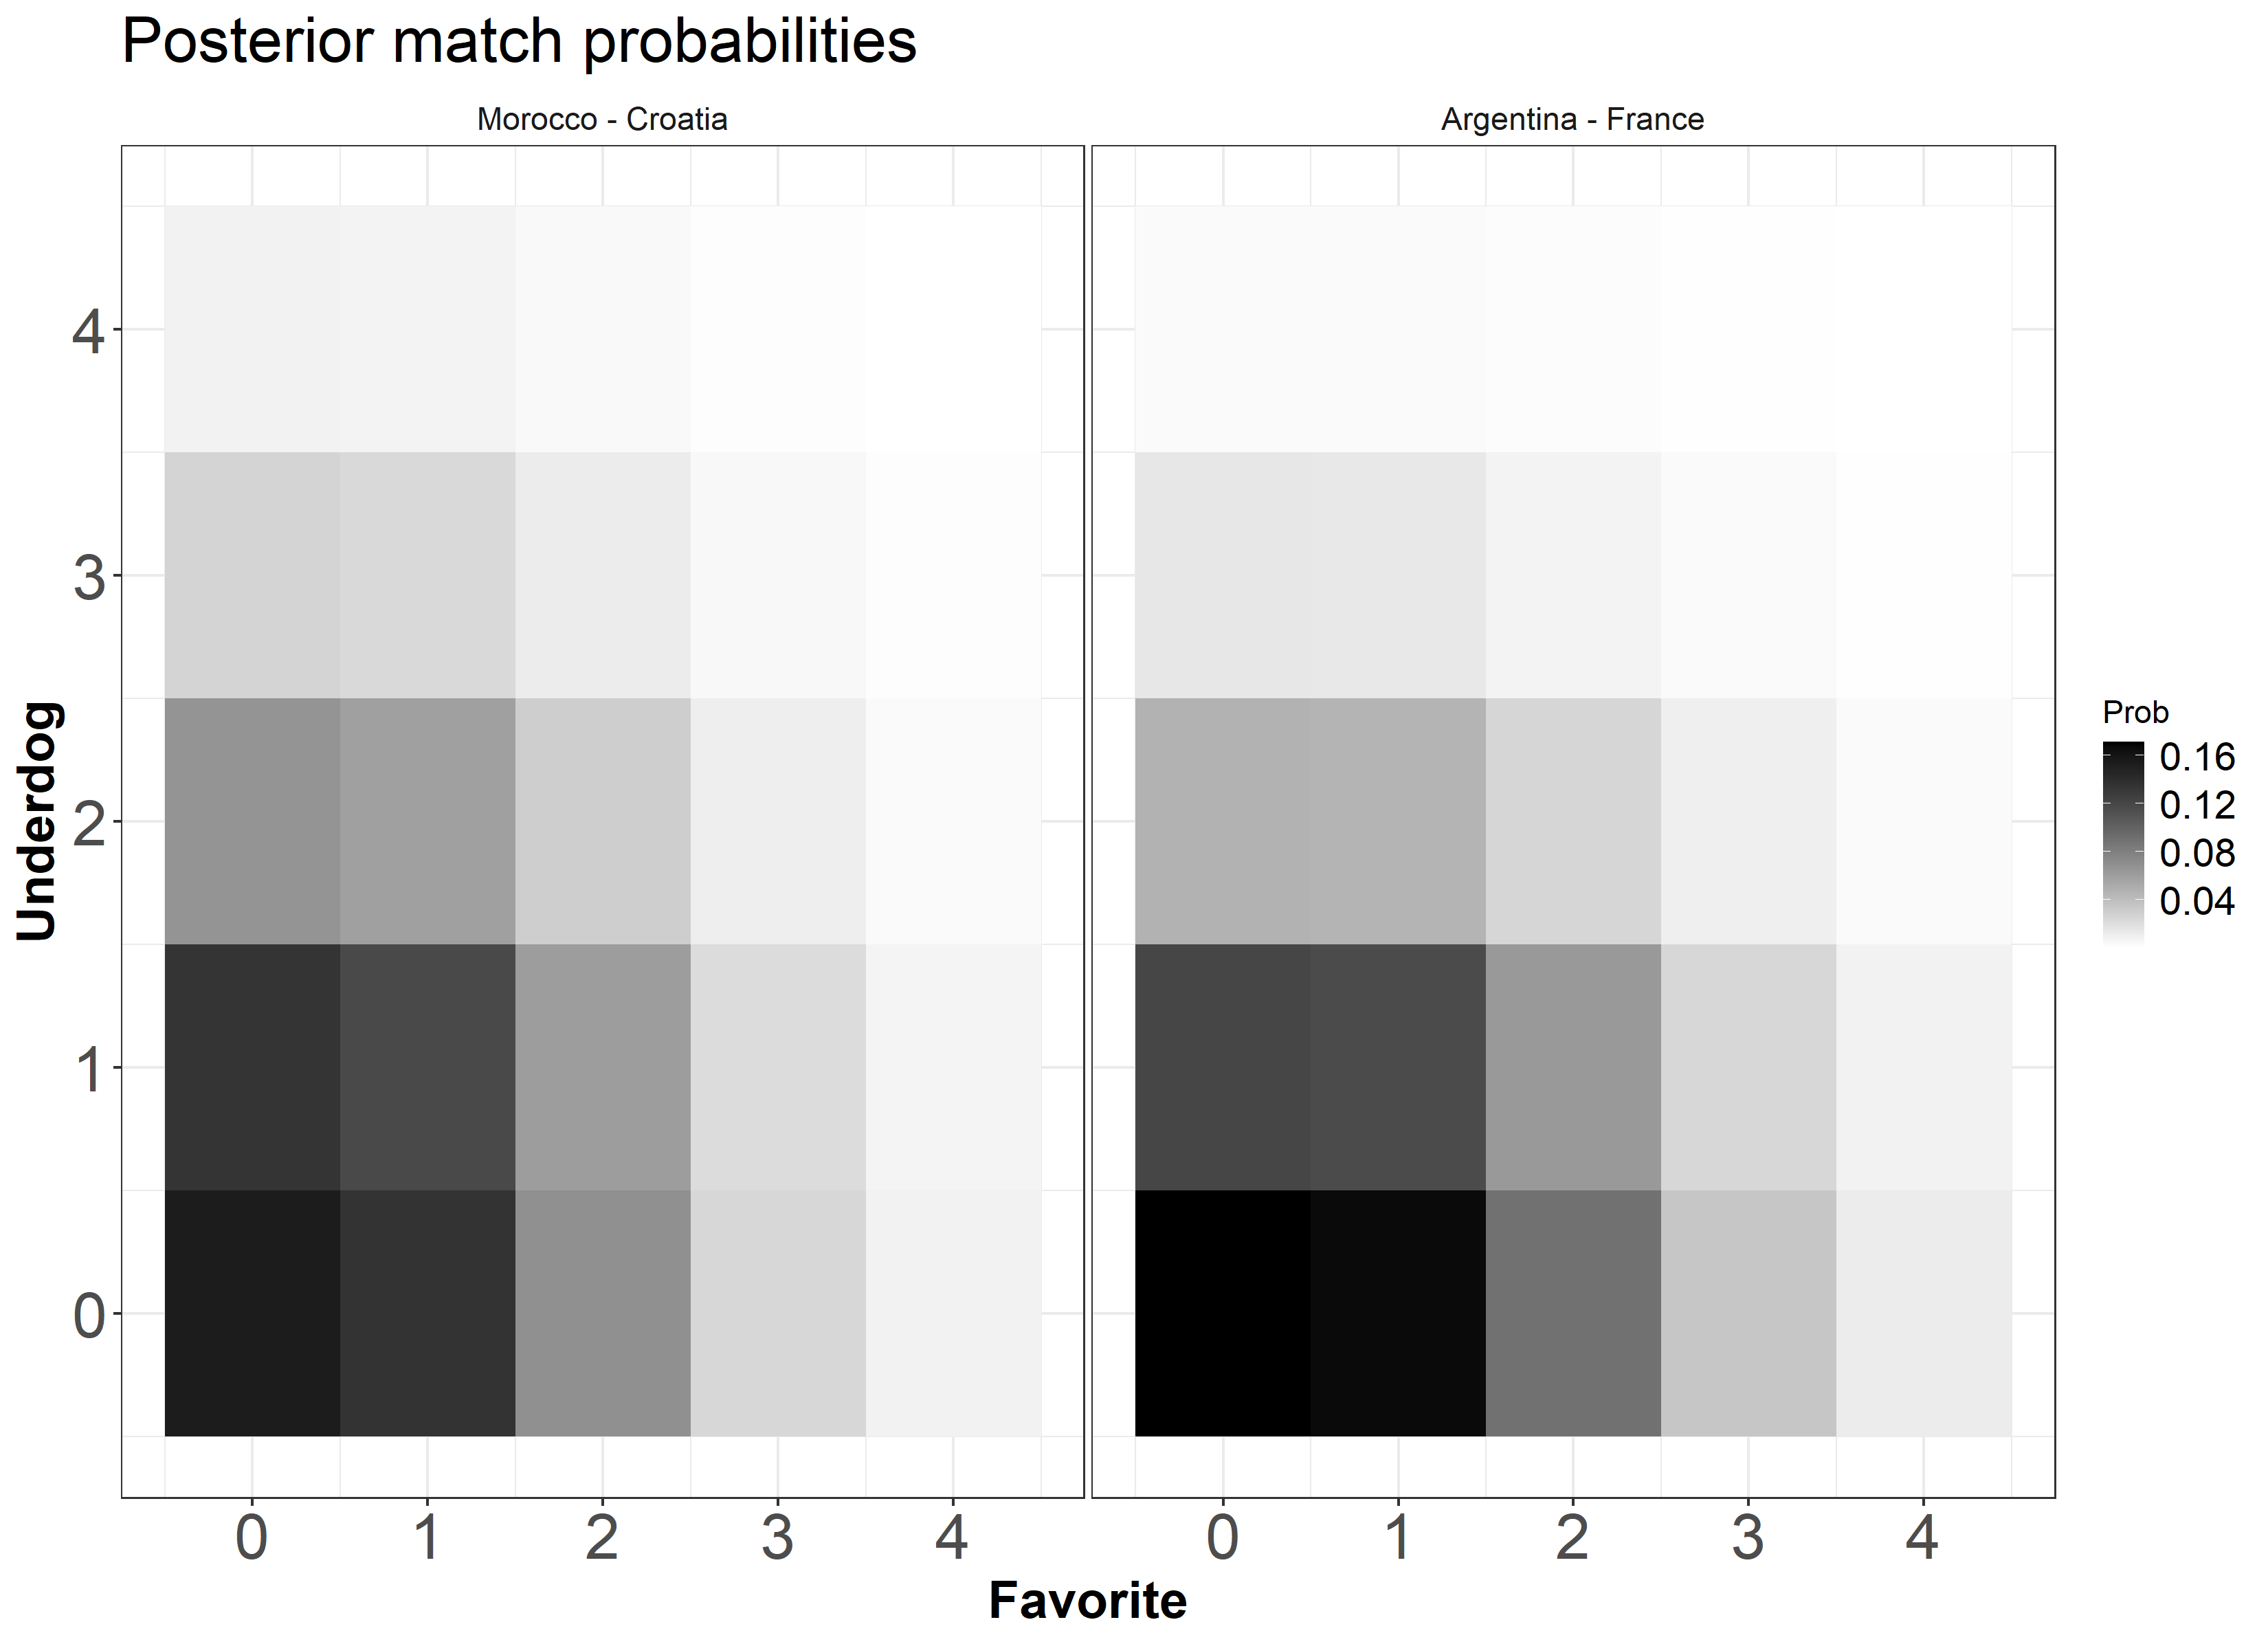
\includegraphics[width=0.8\linewidth]{figs/data2-1} \end{center}

\end{document}
